\chapter{Related Work}

Within the research field of indoor localization there are generally two approaches that use sensors on the user or machine to localize them, one that is infrastructure dependent and the other that is not. Solutions have also been presented that use a combination to try and improve localization \cite{Gu2019}.
The infrastructure dependent methods imitate the GPS method on a local scale. Here they often replace the GPS constellation with signal producing devices available within the indoor environment. Examples of such systems are  wireless fidelity(Wifi), Bluetooth, wireless sensor networks (WSN), and ultra wide band (UWB) \cite{Wu2019,Jackermeier2018,Davidson2017}. These solution naturally only in work in buildings with the installed equipment, requiring some initial investment and setup.\\
The infrastructure independent solution generally leverage sensors that do not need to receive signals from external devices. Such solutions include the use of cameras and inertial sensors. Camera based systems recognize features in the video feed, and combined with known characteristic of the camera and features found in a previous frame, displacement can be determined \cite{Gu2019}. For portable devices continuous use of a camera is not beneficial for battery life, limiting the time duration in which this method can be used.these sensors are \ac{MEMS}, which consist of triaxial orthogonal accelerometers and gyroscopes, and can include a triaxial magnetometer \cite{Yang2014}


\section{Pedestrian Dead Reckoning}
%TODO: this section looks too much like the paper it is from
Inertial Pedestrian Dead Reckoning (PDR) is a positioning technique whose advantage lies in that it only requires MEMS IMU sensors, which can easily be carried by a pedestrian. The output of the system will be the relative position change from a start point, known as dead reckoning. Within PDR there are two methods, namely Inertial Navigation Systems (INSs) and Step and Heading Systems (SHSs).\\
The INS mechanism integrates the IMU signals and is the implementation used most often within research \cite{Diez2018b}. With INS the position error grows cubically with time, due to the signal to noise ratio inherent to MEMS IMU sensors\cite{Harle2013}. In order to compensate this error it is preferable  that the IMU sensor is mounted on the foot, as will be explained in \cref{sec:INS}. This placement requirement may limit the usability. \\
SHS is based on integrating the displacement vectors associated with each step taken during pedestrian locomotion. One advantage of the SHS implementation is that the position error is also proportional to the number of steps taken, but without the preference of using foot-based sensors, allowing for other sensor placements. \\
An overview of the different components required by the two PDR systems can be found in \cref{fig:SHS_INS_diagrams}.\\ Many PDR methods accumulate error with time and are therefore not ideal for long-term pedestrian tracking \cite{Hardegger2012}. Drift reduction methods can be used to try and compensate this error in order to allow for long term tracking \cite{MunozDiaz2019a}, as also shown in the diagrams. This section will outline the different PDR methods and focus on a SHS approach to indoor localization.

\newpage
\begin{figure}[H]
	\centering
	\begin{subfigure}[t]{.7\textwidth}
		\centering
		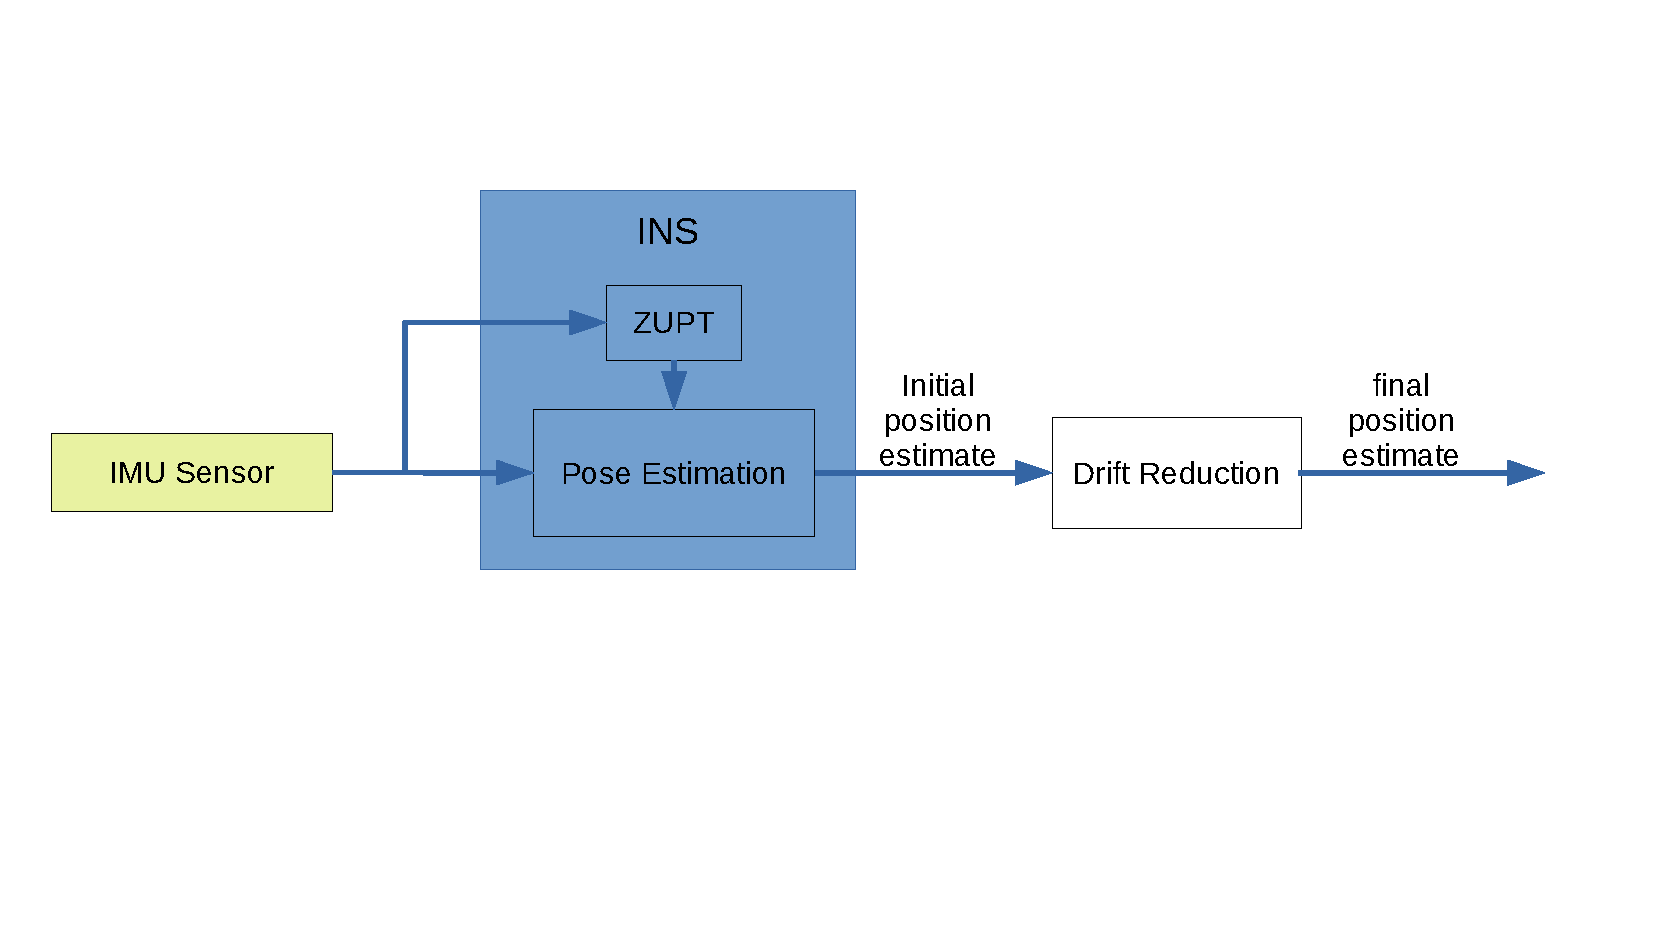
\includegraphics[trim=20 140 50 80, clip, width=\linewidth]{images/INS_diagram}
		\caption{\ac{INS} pedestrian dead reckoning}
		\label{fig:ins_diagram}
	\end{subfigure}\\
	\begin{subfigure}[t]{0.7\textwidth}
		\centering
		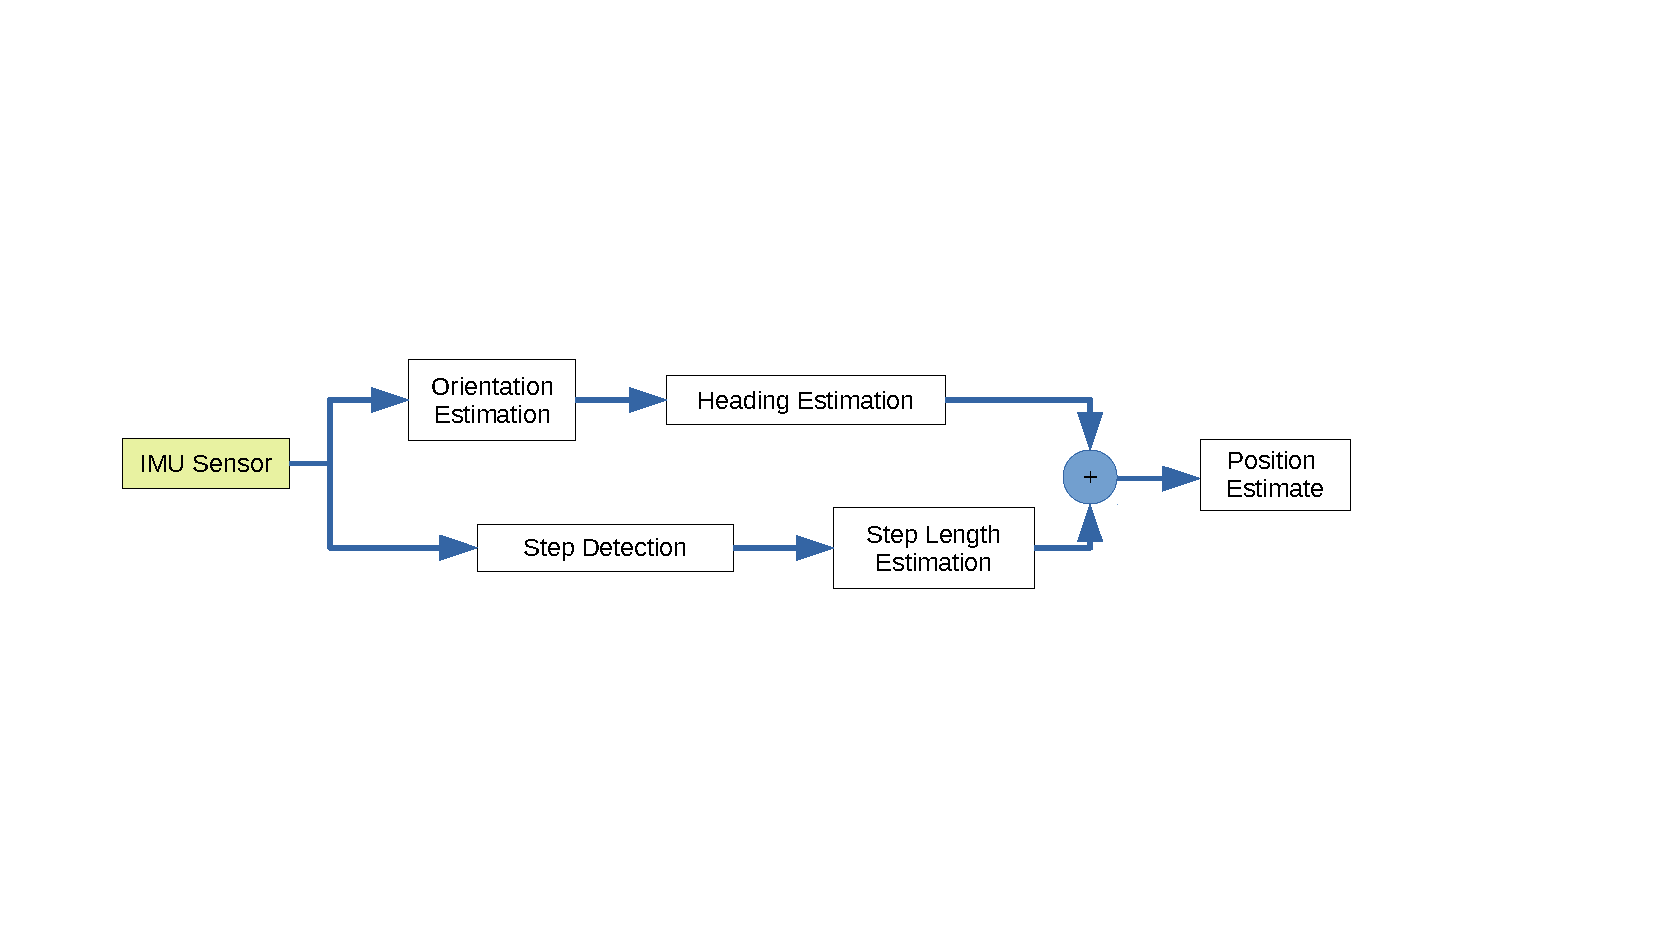
\includegraphics[trim=40 120 40 80, clip,width=\linewidth]{images/shs_diagram}
		\caption{\ac{SHS} pedestrian dead reckoning}
		\label{fig:shs_diagram}
	\end{subfigure}
	\caption{SHS and INS components}
	\label{fig:SHS_INS_diagrams}
\end{figure}
     
\subsection{Inertial Navigation System}
\label{sec:INS}

An \ac{INS} estimates pose, consisting of orientation and position, using sensor fusion algorithms. These methods are directly applied to the signals generated by MEMS IMU sensors \cite{Wu2019}. Examples of sensor fusion algorithms are the Extended Kalman Filter (EKF) and Complementary Filter (CF) \cite{Kok2017}. Sensor fusion algorithms can estimate position and orientation by integrating acceleration twice and integrating angular velocity once, respectively. This integration, in combination with the effects of noise and bias found in MEMS IMU, causes estimation errors to grow cubically with time for INS \cite{Harle2013}. \\
\newline
A technique frequently used to compensate the built up error in INS is zero velocity update (ZUPT) and zero angular update (ZARU) \cite{Harle2013}. It utilizes the ability to detect time periods in which the sensor is stationary during locomotion. Once detected, ZUPT uses the assumption that speed and angular velocity are zero at that time moment \cite{Wu2019,Harle2013}. this a form of pseudo-measurement. This is because the stationary phase is detected, with zero velocity being implied by the assumption, which is not an actual measurement. Comparing the assumption with the output of the sensor fusion algorithm, an error can be calculated and used to compensate the sensor fusion estimate. This process is generally known as a measurement update and would occur every time a stationary period is detected.\\
\newline
Detecting brief stationary time periods in pedestrian IMU data is done easiest when the sensor is placed on the foot. This is because a stationary period is much more pronounced in accelerometer data when the sensor is placed on the foot \cite{Yu2019,Wu2019}.  When walking a foot periodically returns to a stationary state and stays there for a brief period of time approximately 0.1 to 0.3 seconds \cite{Ren2016a}. This has lead to most \ac{INS} research being foot-sensor based \cite{Diez2018,Wu2019}.  \citet{Solin2018a} overcome this preference for a foot based system with a combination of several pseudo measurements, loop closure and position fixes, opening up new possibilities for implementing INS in realistic smartphone use cases.\\
%The highest accuracy in PDR has been reached with INS in combination with ZUPT \cite{Hardegger2012}.
Since the majority of research uses foot mounted systems to implement ZUPT for INS \cite{Wu2019}, it suggest that SHS could be more appropriate for other sensor placements. This is therefore also relevant for PDR in realistic smartphone use cases, since these device are generally not carried in one specific way. Considering this, a focus will be put on implementing a SHS system with the potential to handle different carrying modes. \\


\subsection{Step and Heading System}
\label{sec:rw-SHS}
\ac{SHS} is a form of dead reckoning that identifies steps and their length, and the heading in which the pedestrian is moving. This position estimation can be represented by \cite{MunozDiaz2019}
\begin{equation}
	\label{eq:SHS_dynamic_model}
	\left(\begin{array}{l}
		x_t \\
		y_t
	\end{array}\right) 
	=
	\left(\begin{array}{l}
		x_{t-1} \\
		y_{t-1}
	\end{array}\right) 
	+l_{t} \left(\begin{array}{l}
		\cos \left(\theta_{t}\right) \\
		\sin \left(\theta_{t}\right)
	\end{array}\right)
\end{equation}

where $x_{t}$  and  $y_{t}$ represent the position in the $x$-axis and $y$-axis at time  $t$, respectively. $l_{t}$ stands for the step length, while $\theta_{t}$ is the heading of the pedestrian at time $t$.
There are three components need to apply this system. These are walk and step detection, step length estimation, and step heading estimation.


\subsubsection{Walk and Step Detection}
\label{sec:rw - step detection}
Walk detection is determining from sensor data whether a walking activity is being performed. Step detection is deciding when during the walking activity a step is taken. \\
Techniques such as feature classification, frequency domain analysis, and time domain thresholding can be used to detect the two activities. An overview of some techniques  is  shown in \cref{fig:step_detection_options} and summarized in \cref{tab:step_detection_comparison}. %The reader is referred to \cite{Brajdic2013} for a detailed explanation of each solution.

Naturally, each form of analysis for walk and step detection has its advantages and disadvantages.\\
Time domain analysis often uses acceleration norm, making it robust to sensor orientation \cite{Davidson2017}. Its most simplest form, thresholding, is simple to implement. The problem with thresholding is that it is difficult to determine the optimal threshold, as it can vary between users, surfaces and even shoes \cite{Brajdic2013}. \\
Similarly to time based methods, the periodicity in the norm of acceleration during locomotion is frequently invariant to sensor placement. This therefore also making frequency analysis robust to sensor orientation. Frequency methods have the disadvantage that they are only able to detect periodic motion. 
For both frequency and time domain based analysis, it is possible that certain motions, aside from the desired motion, can cross the threshold and generate false positives. In addition frequency analysis and template matching will have a certain computational overhead to consider \cite{Davidson2017, Harle2013}. \\
Feature classification methods have the advantage that they can determine relations from labeled data automatically, removing a need for humans to define them. This is also a disadvantage as it requires labeled data, the gathering of which can be a labour intensive process. Furthermore, the relationships they determine will depend on the data gathered. This may lead to person dependent performance. In addition, certain classification methods may require significant processing power, limiting the platforms on which it can perform.

\begin{figure}[]
	\centering
	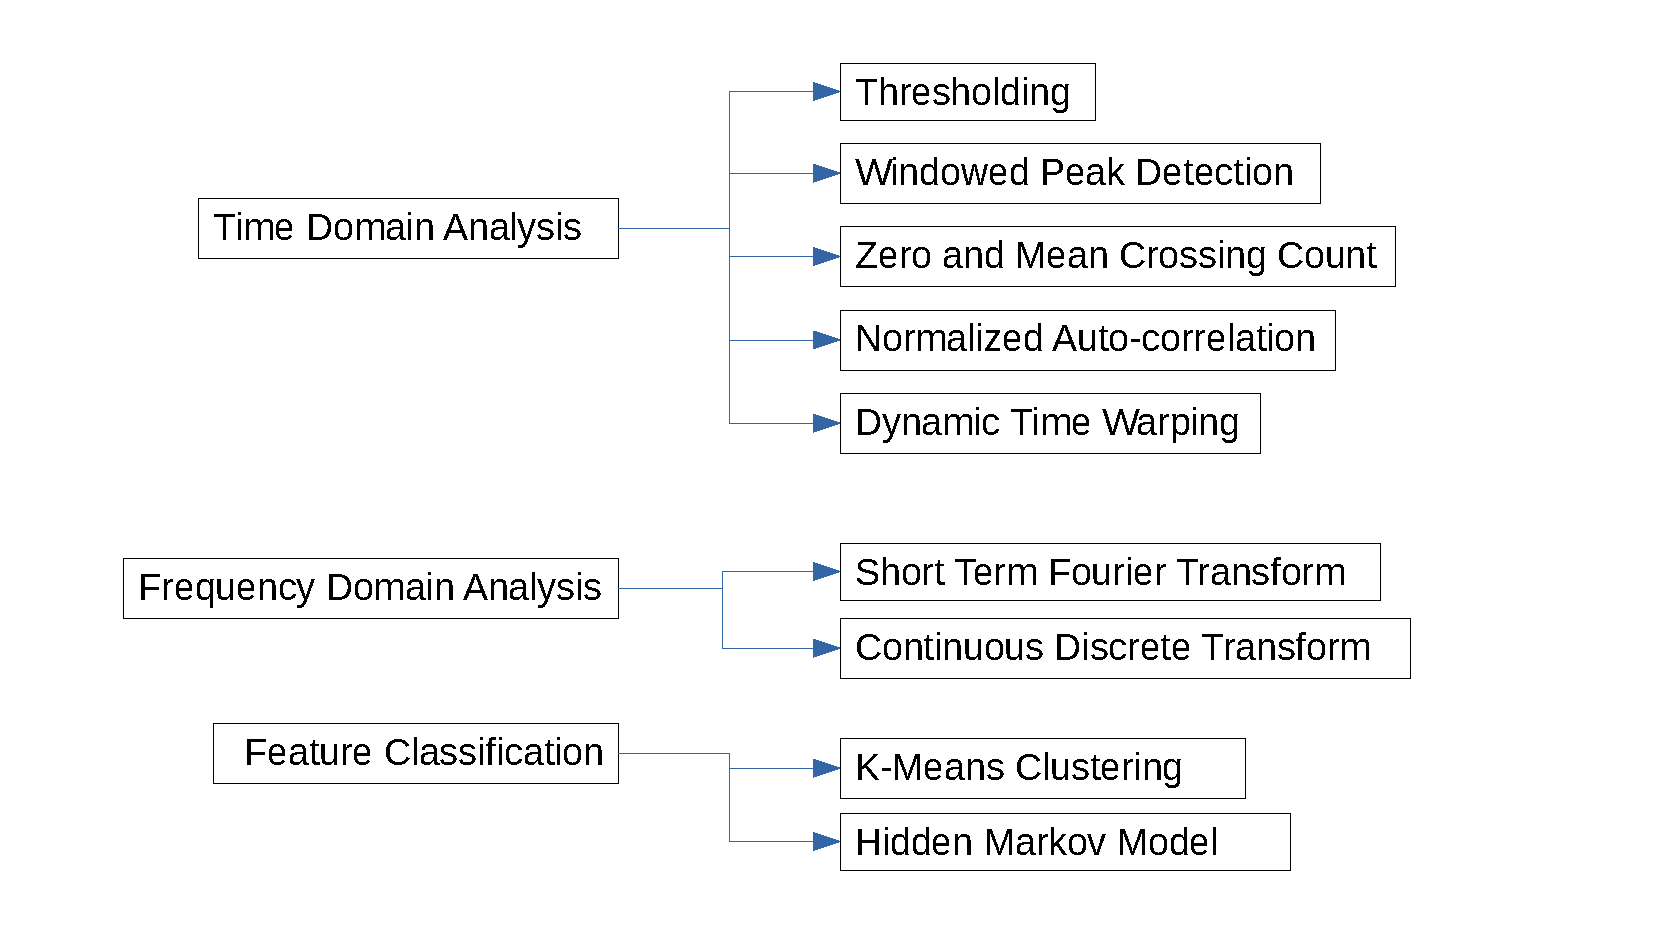
\includegraphics[trim=0 15 0 20, clip,width=0.7\linewidth]{images/step_detection_options}
	\caption{Overview of walk and step detection methods}
	\label{fig:step_detection_options}
\end{figure}

In \cite{Brajdic2013}, a variety of algorithms for both walk detection and step detection on unconstrained smartphones are tested and compared. The paper reviews techniques with different levels of complexity from a variety of different papers. In order to compare the different techniques, \citet{Brajdic2013} collected a large dataset from 27 test subjects leading to 130 recordings was made. Each subject held the smartphone in six different carrying modes: in 
hand in front of user (idle and with device interaction), in a front pocket, in a back pocket and in a handbag or backpack. A ground truth was generated by video recording each session and manually counting the amount of steps taken. Using this dataset a comparison is made between the nine algorithms, 
\newline
The paper concludes that for the generated dataset, the best step counting results were obtained using the windowed peak detection, hidden Markov model and continuous wavelet transform. Each had a median error of about 1.3\%.\\
Considering the relative simplicity of the technique, the authors recommend that the windowed peak detection is the most efficient algorithm. The best walk detection algorithms were thresholds on either standard deviation or signal energy,  short-term Fourier transform, and normalized autocorrelation.\\
\citet{Salvi2018} build upon the conclusions and recommendations of \citet{Brajdic2013}, with the aim of further optimizing the windowed peak detection algorithm and its parameters. The algorithm is based on the approach of \citet{Palshikar2009} and consists of 5 stages run in series. These are pre-processing, filtering, scoring, detection and post processing, as can be seen in the blue squares of \cref{fig:stepdetection} . To optimize the algorithm, different combinations of stage components were compared. A custom made, electronic ground truth device is worn by test subjects for easy comparison with the different combinations. A dataset of 36 recordings was made,  where three researchers walking for two to three minutes with the phone held in six different carrying modes. This includes in hand, in a front pocket, in a back pocket, in an armband, in a shoulder purse, and in a neck pouch on a string. Each set contains around 2.5 minutes of accelerometer and ground truth data. An exhaustive grid search across the parameter space was performed to find the optimal set parameters for step detection. An overview of the optimal parameters can be found in \figref{fig:stepdetection}. Using these parameters an average accuracy of $95\% \pm 4.5\%$ was reached for the different carrying modes.


	\begin{table}[h]
		\centering
		\footnotesize
		\begin{tabularx}{\linewidth}{@{} P{17mm} L}
			\toprule
			\thead[lb]{Technique}	&   \thead[c]{Explanation}	\\
			\midrule			
			Threshold & Acceleration magnitude is monitored for the passing of certain values or sign changes, in the case of Zero Crossing method \cite{Davidson2017,Harle2013}. Typically determines when foot is on the floor \cite{Harle2013}, but has also been applied to pitch angle of upper leg, where the sensor has been placed \cite{Diaz2014a}. In some instances the thresholds are altered adaptively, for example through different motion mode detection or information gathered from the previous step \cite{Wu2019}.\\ \cline{1-2}
  (Windowed) Peak Detection & Recognizes local maximum or minimum on acceleration magnitude caused by foot impact on the floor, often within a sliding window \cite{Susi2013}. Generally combined with thresholding, which is one of the simplest combination used with \ac{SHS} \cite{Davidson2017}. \\ \hline
  Auto-correlation (Template Matching) &  Finds correlation of a signal with a time shifted copy of itself. It leverages the strong cyclic nature of bipedal locomotion \cite{Harle2013}. Since the lag for highest correlation is not known beforehand, an interval is often swept and correlation values compared. \\ \hline
  Dynamic Time Warping & Similar to autocorrelation, it measures the similarity between two waveforms from accelerometer data \cite{Davidson2017}, These waveforms can both come from the data or one could be a stride template generated offline. A non linear mapping between the two methods is made, resulting in a DTW distance. A smaller distance indicates higher similarity \cite{Davidson2017}.  \\ \hline
  Short Term Fourier Transform & Transforms acceleration signal  of successive windows of data into the frequency domain. For a spectral analysis, a subset containing a stride (two steps) is required to determine the frequency \cite{Harle2013}.  \\ \hline
  Wavelet Decomposition & Acceleration magnitude is split into low and high frequency components, from which the dominant frequency is assumed to be the walking frequency. Iterating this process on the resulting low frequency signal approximation, a smoother shaped dominant low-frequency signal is generated. The frequency of this signal corresponds to walking cadence \cite{Davidson2017}. \\ \hline	
  Hidden Markov Model & Uses gait cycles segmented into different states of a state machine, to determine if a step has been taken \cite{Ren2016a}. Thresholds can be used to induce a state change. If a full state machine cycle is achieved, a step is detected.\\ \hline
  K Nearest Neighbours & Uses labeled data containing features from successive time windows and compares a new time window with its features. It finds the labeled data whose features are most similar. This new set recieves then recieves its label. \\
			\bottomrule
\end{tabularx}
		\caption{Overview of different step detection methods}
		\label{tab:step_detection_comparison}
\end{table}
\restoregeometry


\subsubsection{Step Length Estimation}
In order to generate a displacement vector from step detection the step length must be estimated. \citet{Collins2013a} found that increasing step speed leads to larger step lengths, while step speed can have slow and spontaneous fluctuations depending on the motion mode. In addition, step size depends on the physical characteristics of the user and on their walk strategy, which can be different per individual \cite{Diez2018}. These discrepancies indicate that using a simple average step length for every pedestrian could result in quick accumulation of error. 

\citet{Diez2018} categorizes step length estimation methods into integration based and model based methods. \\
Theoretically, the double integration of the IMU acceleration signal is the best approach to step size estimation, using the INS approaches outlined in chapter \secref{sec:INS}. This would give a direct measurement of displacement. It does not require any modeling, assumptions, or person specific calibration \cite{Diez2018}. However, since it would be an INS approach, it suffers from the same drift problems and would require the same solutions. Therefore this approach benefits from having the sensor to be located on the foot. \\
Analytical models can be made of human mobility based on geometrical relationships of body composition, angles and displacement of body parts. One of the largest disadvantages of a model based approach is that human proportions are not uniform, requiring approximations and/or some form of calibration for the model to be accurate.


\citet{Vezocnik2019} compared different existing step length estimation algorithms. The review focuses on the methods applicable to smartphone use. This means methods that do not require training and do not require the sensor to be placed on the foot. This therefore excludes machine learning and INS systems. The models used are either based on an inverted pendulum model or relate predictors to step length. Example of step length predictors are step frequency and acceleration range within a step. The robustness of the methods were tested by having the smartphone in different carrying modes. This includes front pants pocket, in-hand while reading, in-hand while  swinging carrying arm; and in a bag. Furthermore, a comparison was made between the use of global variables, which are variables constant for every user, and personalized variables, where they are tuned per user. The comparison concludes that for global variables the method from \cite{Tian2016} was best, defined as

\begin{equation}
	\label{eq:Tian2016_sle}
	\text{step size} = K \cdot h \cdot \sqrt{F}.
\end{equation}

Here $K$ is a tunable parameter, $h$ is the height of the user and $F$ is the step frequency. This method reported an average error of  4.59 \% for personalized variables and 6.96 \% for global ones. For personally tuned variables the method of \cite{Weinberg2002} was best. This is a n inverted pendulum model in which the human center of mass is used, located approximately at the pelvis. The center of mass rotates as an inverted pendulum when taking a step. This is followed by a forward horizontal displacement when both feet are on the ground \cite{Diez2018}. The model is defined as 

\begin{equation}
	\text{step size} =K \sqrt[4]{A_{\max }-A_{\min }}.
	\label{eq:weinberg_stepsize}
\end{equation}

Here $A_{\max}$ is the largest measured acceleration measured within a step interval, while $A_{\min}$ is the smallest. $K$ is a calibration variable  \cite{Weinberg2002,Diez2018}. The model had an average error of  10.64 \% for global variables and  3.60 \% for personalized \cite{Vezocnik2019}.

\subsubsection{Step Heading Estimation}
Step heading determines the direction of a detected step. It requires the orientation of the sensor in the navigation frame and determining in what direction the sensor is moving in the sensor frame. This provides an estimate in which direction the sensor is moving in the navigation frame.  Step heading estimation is currently the component within SHS whose performance is the most limiting for positioning purposes \cite{Diez2018b, Qian2013,Combettes2017}.
Even though the phone orientation may be known accurately, the direction in which the user is moving is not instantly clear. There are two approaches to determining the heading. The first is knowing beforehand what the orientation of the phone is with respect to heading.  This would constrain the carrying mode that can be used.  With the use of motion classification, this method could be expanded, where different carrying modes can be sensed,which changes the heading accordingly. Heading per carrying mode would need to be derivedbeforehand, through the training of the necessary model. 

\section{Drift Reduction}

\subsection{Pedestrian Dead Reckoning using Activity Recognition}
Research has been done previously on using activity recognition in order to improve indoor localization. \citet{Hardegger2012} created ActionSLAM which uses Simultaneous Localization And Mapping (SLAM) in combination with body mounted error to determine indoor location. It uses a foot mounted sensor to estimate how the user is moving in combination with location-related actions to compensate 



% The Beauregard implementation introduced backtracking, whereby the filter kept a limited history of each particle’s ancestors to allow deletion of an entire trajectory when a particle was killed due to a wall constraint. This is a variant of backward belief propagation also used by Rai et al. [23] and is useful to improve position estimates made in the past when live positioning is not a requirement.
